
\subsection{{\em Fat line}}
Naj bo ${\bf n}$ normalni vektor, ki je pravokoten na ${\bf b}_m - {\bf b}_0$. Definiramo predznačeni razdalji 
\begin{gather*}
d_{\text{max}} = \max _{i=0,\ldots ,m} ({\bf n}\cdot ({\bf b}_i - {\bf b}_0)),\\
d_{\text{min}} = \min _{i=0,\ldots ,m} ({\bf n}\cdot ({\bf b}_i - {\bf b}_0)).
\end{gather*}
Množico $\mathcal{L}$, ki ga sestavljajo točke, ki so od premice ${\bf b}_0{\bf b}_m$ oddaljene kvečjemu za $d_{\text{min}}$ oz. $d_{\text{max}}$ imenujemo {\em fat line}. Krivulja ${\bf g}$ je vsebovana v $\mathcal{L}$, saj je v $\mathcal{L}$ vsebovana njena konveksna ovojnica.
\begin{figure}[!h]
    \centering 
    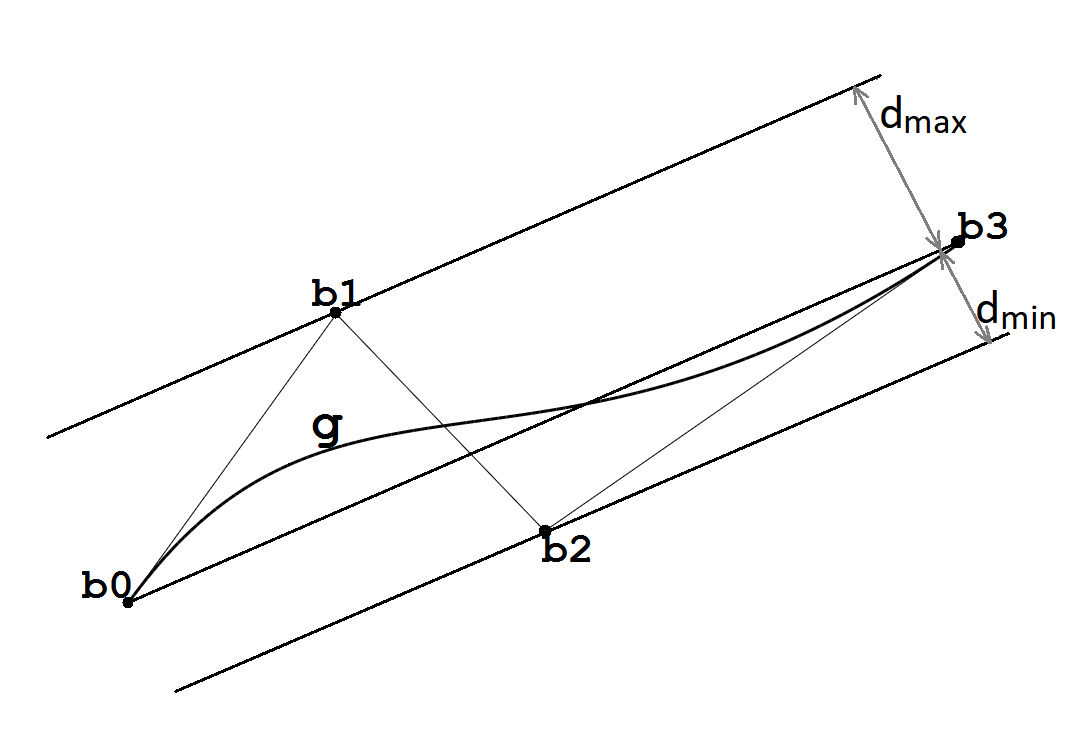
\includegraphics[width=0.5\textwidth]{fat_line}
    \caption{Krivulja {\bf g} in {\em fat line.}}
  	%\caption{{\em Fat line $\mathcal{L}$}.}
  	\label{slika3}
\end{figure}